\documentclass[12pt,a4paper,oneside,openany,parskip=full,parindent=full]{book}
\usepackage[T1]{fontenc}
\usepackage[utf8]{inputenc}
\usepackage[polish]{babel}
\usepackage{graphicx}
\usepackage{times}
\usepackage{indentfirst}
\usepackage[left=3cm,right=2cm,top=2.5cm,bottom=2.5cm]{geometry}
\usepackage{natbib}
\usepackage{color}
\usepackage{tikz}
\usepackage{url}
\usepackage{dirtree}
\edef\restoreparindent{\parindent=\the\parindent\relax}
\usepackage{parskip}
\restoreparindent
\usepackage{listings}
\usepackage{enumerate}
\usepackage{color}


\definecolor{dkgreen}{rgb}{0,0.6,0}
\definecolor{gray}{rgb}{0.5,0.5,0.5}
\definecolor{mauve}{rgb}{0.58,0,0.82}

\lstset{frame=tb,
  language=Python,
  aboveskip=3mm,
  belowskip=3mm,
  showstringspaces=false,
  columns=flexible,
  basicstyle={\small\ttfamily},
  numbers=none,
  numberstyle=\tiny\color{gray},
  keywordstyle=\color{blue},
  commentstyle=\color{dkgreen},
  stringstyle=\color{mauve},
  breaklines=true,
  breakatwhitespace=true,
  tabsize=3
}


\frenchspacing
\linespread{1.5}
\addto\captionspolish{%
\renewcommand*\listtablename{Spis tabel}
\renewcommand*\tablename{Tabela}
}

\frenchspacing

\begin{document}

\begin{center}

\vspace{1cm}

Studium licencjackie
\end{center}

\vspace{1cm}

\noindent Kierunek: Informatyka

\noindent Specjalność: Bazy danych i technologie internetowe

\vspace{1cm}

{
\leftskip=10cm\noindent
Michał Polakowski\newline
Nr albumu: 203446\newline
Karol Chmielewski\newline
Nr albumu: 246668\newline
Michał Pydyszewski\newline
Nr albumu: \newline
Bartłomiej Pysiak\newline
Nr albumu:
}

\vspace{2cm}

\title{Praktyczne zastosowanie web scrapingu do tworzenia użytkowych aplikacji internetowych}
\makeatletter

\begin{center}
\LARGE\bf
\@title
\end{center}

\vspace{2cm}

{
\leftskip=10cm\noindent
Praca licencjacka\newline 
napisana w~Instytucie Matematyki, Fizyki i Informatyki\newline
pod kierunkiem naukowym\newline
dra Włodzimierza Bzyla

}

\vfill

\begin{center}
Gdańsk, \the\year
\end{center}
\thispagestyle{empty}

\clearpage
\thispagestyle{empty}
\clearpage

\tableofcontents

\clearpage
\chapter*{Strzeszczenie}

Nasza praca opisuje aplikację webową służącą jako pomoc w dopasowaniu za pomocą web-scrapingu elementu garderoby do najlepszych propozycji dostępnych w sklepach internetowych. 

Naszym celem było ukazanie w jaki sposób można zaimplementować web-scraping w aplikacji internetowej.

Web-scraping oparty jest na frameworku Scrapy, aplikacja zbudowana jest przy użyciu frameworka webowego Django, anonimizacja użytkownika i optymalizacja wydajnościowa jest możliwa dzięki serwerowi NGINX. Wszystkie zadania są obsługiwane przy użyciu kolejek dzięki Celery, a zbierane informacje są zapisywane w MongoDB oraz PostgreSQL. W pracy opisujemy działanie każdego z modułów, oraz przedstawiamy moralne aspekty web-scrapingu.
\chapter{Wprowadzenie}

Pomysł na naszą aplikację narodził się podczas odbywanych przez nas licznych wizyt w galeriach handlowych, gdzie zauważyliśmy, jak dużo czasu, wysiłku i pieniędzy ludzie poświęcają aby do posiadanej odzieży dopasować nowe elementy garderoby.

Na taki stan rzeczy składa się kilka czynników. Pierwszym z nich jest dostępność produktów. Wybór konsumenta ograniczony jest przez wyposażenie sklepów na terenie galerii. Ponadto, konsument ma tendencję do kupienia produktu, który w jego mniemaniu jest nabliższy temu, czego oczekiwał, lecz często nie dokładnie taki. To pokazuje nam kolejny problem - konsument nie pozytkuje swoich pieniędzy najlepiej, jak to możliwe. Nie sposób jest porównać wszystkich przedmiotóœ z puli potencjalnych dopasowań, ponieważ są one rozproszone po różnych sklepach, a często galeriach a nawet miastach. Trzecim czynnikiem jest czas poświęcony na wybieraniu potencjalnych dopasowań, ponieważ koniecznym jest fizycznie udać się do sklepów.

Jednym z rozwiązań problemu braku czasu jest zatrudnienie stylisty, który podpowie, które dopasowanie jest najlepsze, lecz jest to kosztowna usługa, na którą nie każdy może sobie pozwolić.

Odpowiedzią na te problemy jest nasza aplikacja. Po wprowadzeniu w pasku wyszukiwarki produktu, prezentowana jest użytkownikowi lista najlepiej skomponowanych do niego artykułów wraz z linkiem do sklepu, zdjęciem oraz ceną.
Wystąpienie na liście propozycji dopasowania podyktowane jest jego popularnością oraz częśtotliwością doboru wśród innych użytkowników systemu.
Pozwala to na oszczędzenie czasu poprzez możliwość porównania bez wychodzenia z domu.
Aplikacja przyczynia się również do oszczędności pieniędzy, ponieważ niejako eliminuje potrzebę zatrudniania stylisty.

Produkt działa z wykorzystaniem web-scrapingu opartego na pythonowym frameworku Scrapy.
Poniższy diagram przedstawia po krótce proces działania wspomnianego modułu.
ZDJĘCIE

Wyszukiwania są cachowane na serwerze pośredniczącym, co pozwala użytkownikowi na szybsze wyszukiwanie i płynniejsze korzystanie z aplikacji.
Zasoby statyczne takie jak zdjęcia pobierane są z serwera pośredniczącego, a nie z domeny docelowej.

Dodatkowym atutem korzystania z serwera pośredniczącego jest ukrycie prawdziwego adresu logicznego użytkownika, dzięki czemu utrudni to reklamodawcom prezentowanie mu reklam, co miałoby miejsce w przypadku bezpośrednich wizyt w poszczególnych domenach sklepów internetowych.sklepach

W projekcie wykorzystujemy load balancing, dzięki któremu ruch będzie rozpraszany na wszystkie węzły, a użytkownik nie odczuje spadku wydajnośći w przypadku wzmożonego ruchu.

Słowa kluczowe: web-scraping, dopasowanie ubrań, stylizacja modowa
\chapter{Django}

Python jest aktualnie jednym z najpopularnijeszych języków programowania na świecie

\section{Popularność}
Pierwszym czynnikiem wpływającym na nasz wybór była popularność frameworka. 
\chapter {Scraper} 

W niniejszym rozdziale zajmę się omówieniem użytych w projekcie zagadnień dotyczących webscrapingu.

Scrapy jest jedną z najpopularniejszych bibliotek pythonowych, które mają za zadanie zbierać informacje ze stron internetowych.
Webscraping oparty jest na pyhtonowym frameworku \emph{Scrapy}, wspieranym przez biblioteki \emph{Splash} oraz \emph{XPath}.
Uzyskiwałem wiedzę posługując się dokumentacjami bibliotek \emph{Scrapy}\footnote{\url{https://doc.scrapy.org}}, \emph{Splash}\footnote{\url{https://splash.readthedocs.io/en/stable/api.html}} oraz \emph{XPath}\footnote{\url{https://doc.scrapy.org/en/xpath-tutorial/topics/xpath-tutorial.html}}.

Skrypt uruchamiany jest na trzech stronach sklepów internetowych: \emph{https://reserved.com, https://zalando.pl, https://domodi.pl}. 
Wykonywanie programu jest podzielone na trzy etapy:
\begin{enumerate}
	\item Po uzyskaniu słów kluczowych program wprowadza w wyszukiwarce strony daną frazę wpisaną przez użytkownika.
	\item Przekierowuje do wszystkich wyników wyszukiwania.
	\item Zbiera oraz zwraca informację z rubryki wygenerowanej dynamicznie przez stronę, która	ma na celu poinformowanie kupującego o rzeczach zakupionych przez innych użytkowników wraz z wyszukiwanym ubraniem.
\end{enumerate}
\section{Opis etapów}

\subsection{Etap 1}
	Aplikacja włącza program scrapingowy za pomocą następującej komendy: \emph{scrapy crawl clothing -a tag=”fraza” -o results.json}.
Oznacza to uruchomienie programu o nazwie \emph{clothing} z parametrem do wyszukania (tag), a rezultat będzie przechowywany do pliku \emph{results.json}.
Po uruchomieniu, do każdej strony internetowej inicjowana jest metoda \emph{search}, która za pomocą \emph{XPath} odszukuje formularz na stronie głównej sklepu, wpisuje interesującą użytkownika nazwę ubrania i wysyła request z żądaniem wyszukania.

\subsection{Etap 2}
	Strona sklepu internetowego zwraca wyniki wyszukiwania. Program zbiera wszystkie linki do wyszukanych ubrań za pomocą \emph{XPath}, który przeszukuje w kodzie HTML odnośniki mające w adresie przekierowującym rodzaj ubrania. Następnie przechodzi do tych stron odpalając kolejną metodę, która zależnie od sklepu szuka w kodzie HTML strony innych struktur.

\subsection{Etap 3}
	Będąc na tym etapie program jest już w dokładnie jednej ofercie zakupu ubrania. Zależnie od strony, skrypt zachowuje się w inny sposób:
\begin{itemize}
	 \item dla stron \emph{reserved} oraz \emph{domodi} od razu następuje przeszukiwanie kodu HTML w celu znalezienia proponowanych rzeczy poprzez znalezienie odpowiedniej struktury
		\begin{itemize} 
			\item dla sklepu Reserved każda oferta przeszukiwania jest umieszczona w znaczniku \textless div\textgreater, a znacznik ten zaczyna się od klasy, która ma nazwę \emph{portrait}. Dla Domodi jest to każdy 	znacznik \textless li\textgreater.
		\end{itemize}
	\item dla sklepu Zalando wyszukiwany jest najpierw tekst \emph{zobacz więcej}. Po znalezieniu tekstu aplikacja przechodzi na tą podstronę, żeby móc wylistować wszystkie ubrania proponowane przez sklep. W przypadku, gdy tekst \emph{zobacz więcej} nie zostanie znaleziony, aplikacja nie zwróci żadnych propozycji ze strony Zalando.\end{itemize}
Program pobiera następujące informacje z propozycji kupna:
\begin{itemize}
	\item adres URL
	\item zdjęcie ubrania
	\item cenę
	\item nazwę ubrania
\end{itemize}
Informacje zapisywane są tylko wtedy, jeśli jest ich cały komplet – powoduje to uniknięcie przedostawania się do wyników niepotrzebnych danych bądź innych przypadkowo pobranych rzeczy.
Zapisywanie odbywa się w formacie json o strukturze słownikowej:
\begin{itemize}
\item[] \emph{\{ClothesName: \{ "image": imageURL, "price": PRICE, "url": URL\}\}}
\item[] \emph{ClothesName} – przechowywany w formacie string; jako wartość zawiera słownik ze szczegółami
\item[] \emph{imageURL} – przechowywany w formacie string; zawiera adres do zdjęcia ubrania
\item[] \emph{PRICE} – przechowywany w formacie string; zależnie od strony może być z końcówką „zł” lub „PLN”
\item[] \emph{URL} – przechowywany w formacie string; zawiera adres do strony sklepu z daną rzeczą
\end{itemize}
Program na bieżąco przesyła taki słownik do pliku wynikowego, z którego dalsza część programu może na bieżąco czytać.


Program, żeby mógł działać na dynamicznych stronach używa biblioteki Splash.
Splash używa funkcji napisanej w języku Lua:
\begin{lstlisting}
function main(splash, args)
          assert(splash:go(args.url))
          assert(splash:wait(0.5))
          assert(splash:set_viewport_full())
          return {
            html = splash:html()}
            end
\end{lstlisting}\footnote{\url{https://splash.readthedocs.io/en/stable/scripting-tutorial.html}
\begin{itemize}
\item[] Splash:go(args.url) przechodzi na stronę podaną w argumencie.
\item[] Splash:wait(0.5) – określa jak długo program czeka na załadowanie strony
\item[] Splash:set\_viewport\_full() sprawia, że wczytywana jest cała strona HTML

Wysyłanie requestów do stron również odbywa się za pomocą metody z biblioteki Splash -- \emph{SplashRequest}, która jako argumenty przyjmuje adres strony, metodę do której ma przejść w następnym kroku oraz argumenty (przekazanie całej funkcji z języka Lua jako parametr).
\end{itemize}
\section{Dlaczego Scrapy}

Scrapy jest stosunkowo dużym frameworkiem skupionym na webscrapingu. Nie jest trudno opanować podstawy -- framework ten jest bardzo dobrze udokumentowany oraz posiada dużo poradników dotyczących pierwszych kroków. Wszystkie te udogonienia pozwalają poznać podstawowe fundamenty Scrapy, które w dużej mierze powinny wystarczyć do większości zadań związanych z webscrapingiem. Posiada własne selektory, dzięki którym można swobodnie poruszać się po stukturze HTML. Jego największą zaletą jest to, że służy jako crawler -- wystarczy podać adres początkowy, a framework będzie w stanie przeszukiwać wgłąb stronę wedle chęci osoby piszącej program.

Przy wielkości opisywanego przez nas projektu oraz przy daleko idących planach rozbudowy aplikacji pisanie crawlera we frameworku w pełni skupionym na scrapingu jest niezbędne do uniknięcia dalszych problemów związanych z obsługą coraz bardziej skomplikowanych stron internetowych.
\subsection{Selektory}

Scrapy implementuje własne selektory pozwalające przeszukiwanie kodu HTML.
Można wydobywać części kodu za pomocą języka XPath oraz poprzez wybieranie kodu CSS, który stylizuje HTML.

W opisywanej aplikacji zdecydowałem się na posługiwanie się językiem XPath -- był dla mnie wygodniejszy i łatwiejszy w nauce.
Przykładowy selektor z napisanego przeze mnie scrapera, który jest używany w naszym programie:
\begin{lstlisting}
response.xpath("//a[./img[contains(@src,.)]]/@href").extract()
\end{lstlisting}
Powyższa linijka oznacza wybranie wszystkich znaczników \textless a\textgreater. Następnym krokiem jest znalezienie takich znaczników \textless img\textgreater, które posiadają w sobie odnośniki do innych stron. 
\emph{Extract()} powoduje, że wszystkie wyniki wyszukiwania pojedynczo będą formatowane jako typ string, który będzie można przekształcić wedle uznania.
Ważnym elementem selektorów jest możliwość wyszukania danej informacji znajdującej się wewnątrz wybranych znaczników.
Za przykład posłuży mi fragment kodu. Ma on za zadanie zebrać wszystkie niezbędne informacje na temat strony \emph{zalando.pl}:
\begin{lstlisting}
        for item in response.xpath("//div[./a[contains(@href,'zalando.pl')]]"):
            url = item.xpath('./a/@href').extract()
            itemImg = item.xpath('.//*/img[contains(@src,.)]/@src').extract()
            price = item.xpath(".//span[contains(text(),'zl')]/text()").extract_first()
            itemName = item.xpath('.//*/img[contains(@src,.)]/@alt').extract()
\end{lstlisting}

Kod ten napisałem sam, za pomocą dokumentacji Xpath oraz Scrapy. Xpath zaczynający się od kropki oznacza, że program zaczyna przeszukiwać od -- podanego w przykładzie wyżej, \textless a\textgreater. Wybierane są tylko hiperłącza posiadające odnośnik do strony zawierającej podstring "zalando.pl".

Finalnie, jeśli zdajemy sobie sprawę które rzeczy Scrapy powinien szukać oraz mamy otwartą stronę z dokumentacją\footnote{\url{https://doc.scrapy.org}}, to napisanie owego crawlera od podstaw, nie znając wcześniej składni, okazuje się stosunkowo proste i przyjemne.

\chapter {Wizualna prezentacja projektu} 

Niniejszy rozdział poświęcony jest przedstawieniu projektu ze strony wizualnej.

Wchodząc na naszą aplikację pierwszym obrazkiem, który nas powita jest strona tytułowa wraz z zablokowanym oknem formularza, w którym będziemy mogli wpisać nazwę ubrania, do którego program będzie szukać dopasowań.

\begin{figure}[h]
    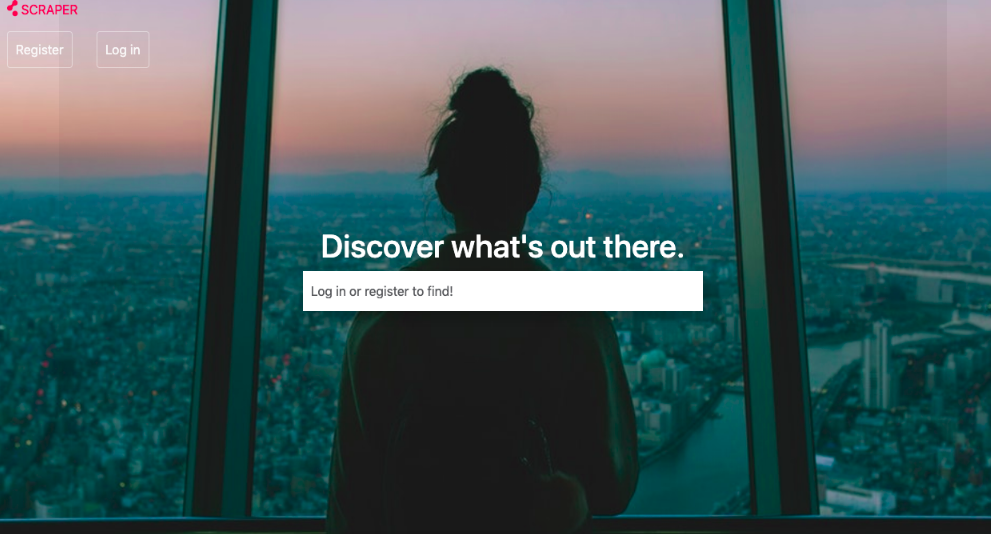
\includegraphics[width=1.10\textwidth]{zdjecia/tytulowa}
    \caption{Strona tytułowa}
\end{figure}

Użytkownik, żeby móc korzystać z aplikacji musi się zarejestrować. W tym celu klika przycisk \emph{Register}, a następnie wypełnia formularz.

\begin{figure}[h]
    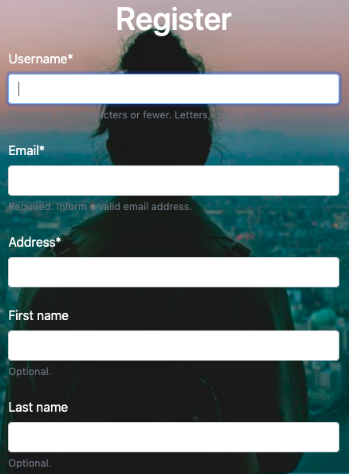
\includegraphics[height=10cm]{zdjecia/registration}
    \caption{Formularz rejestracji}
\end{figure}

\newpage
Następnym krokiem po rejestracji jest logowanie. Używając danych wpisanych podczas rejestracji można zalogować się do systemu.

Od tej chwili użytkownik może korzystać z aplikacji w stu procentach.\newline
Pojawiło się okna \emph{History} oraz \emph {Results}, w których odpowiednio można przeglądać swoją historię wyszukiwań oraz wyniki ostatniego wyszukania.
\begin{figure}[h]
    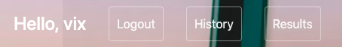
\includegraphics{zdjecia/history_results}
    \caption{Wszystkie okna użytkownika}
\end{figure}

Jeśli przejdziemy do podstrony z historią wyszukiwań, otrzymamy widok z tabelą, która ma dwie kolumny: \emph{Name} i \emph{Date}.\newline
Tabela jest sortowalna, jest możliwość wyszukania na podstawie frazy wpisanej przez użytkownika.
\begin{figure}[h]
    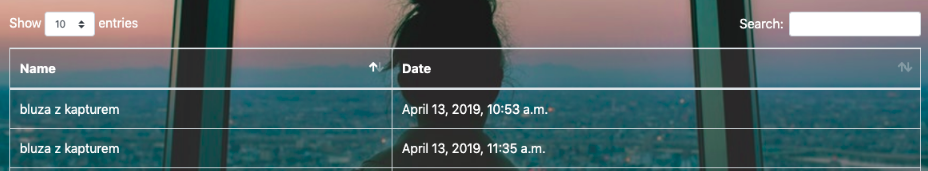
\includegraphics[width=1.10\textwidth]{zdjecia/history}
    \caption{Historia wyszukiwań}
\end{figure}
\newpage
Na stronie głównej zostało odblokowane okno z wyszukiwaniem. W tym celu można wpisać interesującą użytkownika rzecz, a następnie przejść do zakładki results, w której pojawi się tabela z nazwą ubrania, ceną, linkiem do sklepu oraz linkiem do zdjęcia. Tabela jest w pełni sortowalna, można wyszukiwać danej frazie.
\begin{figure}[h]
    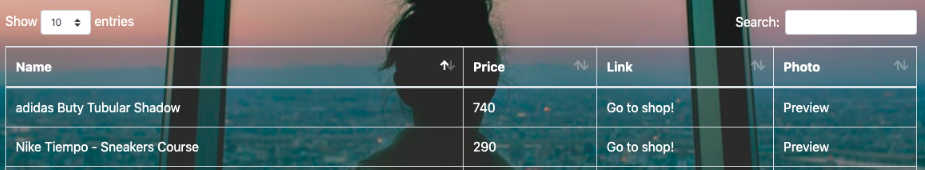
\includegraphics[width=1.10\textwidth]{zdjecia/wyniki}
    \caption{Wyniki wyszukiwań}
\end{figure}

\chapter{Podsumowanie}




\clearpage
\bibliography{main}
\bibliographystyle{ieeetr}

\clearpage


\end{document}
